\section[Расчетная часть]{РАСЧЕТНАЯ ЧАСТЬ}

\subsection{Описание комплекса технических средств системы}

Предполагается, что проектируемое приложение будет использоваться
на мобильных устройствах под управлением операционной системы Android
версии не ниже 4.1.

Для полноценной работы приложения требуется наличие фотокамеры.

\subsection{Организация работы системы}

Рассмотрим несколько диаграмм, разработанных по методологии IDEF,
описывающих работу проектируемого приложения.

% main
На рисунке~\ref{fig:idef0_main} представлена диаграмма декомпозиции
верхнего уровня.

\begin{figure}[h!]
  \centering
  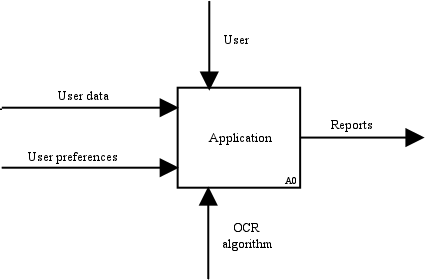
\includegraphics[width=130mm]{pic/idef0_main}
  \caption{Диаграмма декомпозиции \\ верхнего уровня}
  \label{fig:idef0_main}
\end{figure}

Из этого рисунка видно, что на вход приложению подаются финансовые данные
и пользовательские настройки, выходом являются отчеты,
роль механизма выполняет алгоритм распознавания изображений (OCR),
а управления --- пользователь.

\pagebreak
% application
На рисунке~\ref{fig:idef0_app} представлена диаграмма декомпозиции
приложения.

\begin{figure}[h!]
  \centering
  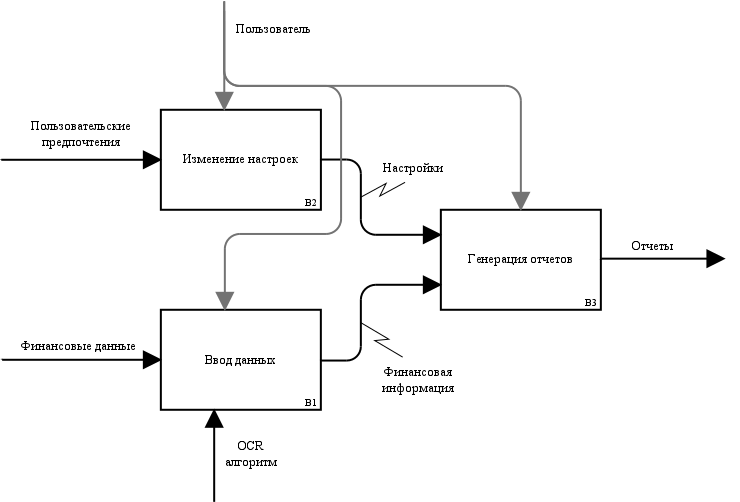
\includegraphics[width=150mm]{pic/idef0_app}
  \caption{Диаграмма декомпозиции приложения}
  \label{fig:idef0_app}
\end{figure}

Из этого рисунка видно, что работу приложения можно разделить
на следующие этапы:
\begin{itemize}
\item настройка приложения;
\item ввод данных;
\item генерация отчетов на основании данных и настроек.
\end{itemize}

\pagebreak
% settings
Рассмотрим подробнее процесс выбора настроек приложения,
представленный на рисунке~\ref{fig:idef3_settings}.
В соответствии с ним, пользователь может изменить список счетов,
добавить или удалить категорию учета, а также выбрать валюту ввода
по умолчанию.

\begin{figure}[h!]
  \centering
  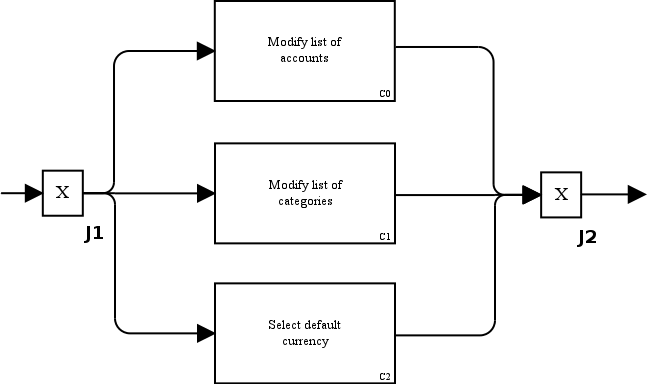
\includegraphics[width=150mm]{pic/idef3_settings}
  \caption{Диаграмма выбора настроек приложения}
  \label{fig:idef3_settings}
\end{figure}

\pagebreak
% input
Рассмотрим подробнее процесс ввода данных,
представленный на рисунке~\ref{fig:idef3_input}.
В соответствии с ним, для ввода данных требуется
ввести сумму вручную либо с изображения, выбрать категорию и дату ввода.

\begin{figure}[h!]
  \centering
  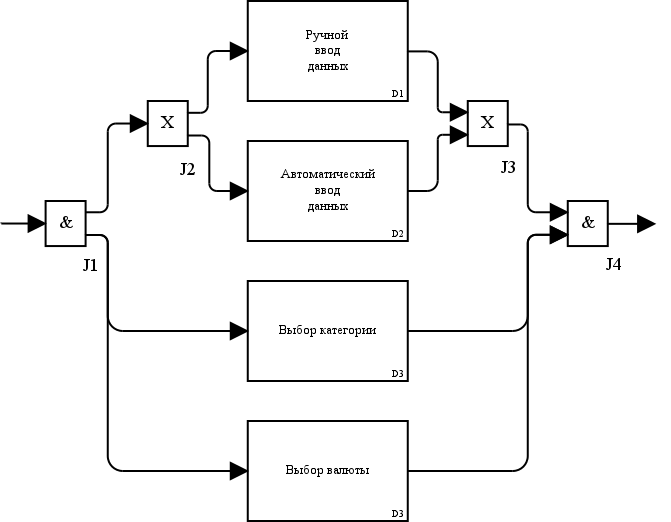
\includegraphics[width=150mm]{pic/idef3_input}
  \caption{Диаграмма процесса ввода данных}
  \label{fig:idef3_input}
\end{figure}

\pagebreak
% input
Рассмотрим подробнее процесс получения отчетов,
представленный на рисунке~\ref{fig:idef3_reports}.
В соответствии с ним, для отчета пользователь должен выбрать
учетный период, счета, валюту и учитываемые категории.

\begin{figure}[h!]
  \centering
  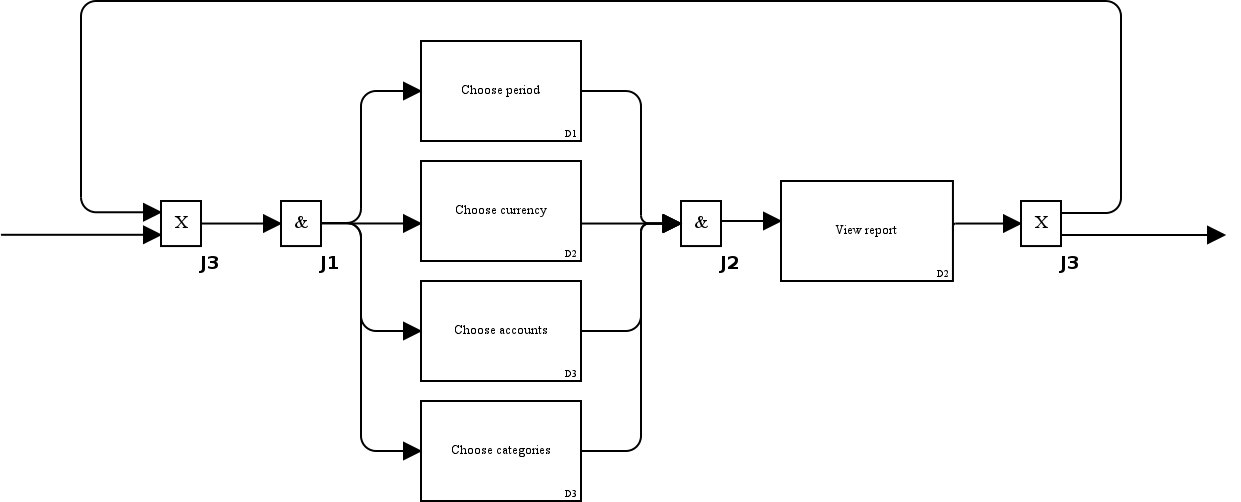
\includegraphics[width=150mm]{pic/idef3_reports}
  \caption{Диаграмма процесса получения отчета}
  \label{fig:idef3_reports}
\end{figure}
